%=========================================================
%               CLASSE DU DOCUMENT
%=========================================================
\documentclass[12pt,a4paper]{article}

%=========================================================
%         ENCODAGE ET POLICES DE CARACTÈRES
%=========================================================
\usepackage[utf8]{inputenc}    % Encodage UTF-8 (inutile avec XeLaTeX/LuaLaTeX)
\usepackage[T1]{fontenc}       % Meilleure gestion des caractères accentués
\usepackage{lmodern}           % Police Latin Modern
\usepackage{times}             % Police Times (à supprimer si tu préfères Latin Modern)

%=========================================================
%                MATHÉMATIQUES
%=========================================================
\usepackage{amsmath}           % Environnements mathématiques avancés
\usepackage{amssymb}           % Symboles mathématiques supplémentaires
\usepackage{amsfonts}          % Polices mathématiques
\usepackage{mathrsfs}          % Police calligraphique (\mathscr)
\usepackage{tkz-tab}           % Tableaux de signes et de variations
\everymath{\displaystyle}      % Affiche toutes les formules en style "display"

%=========================================================
%               MISE EN PAGE
%=========================================================
\usepackage[
    left=1cm,
    right=1cm,
    top=1cm,
    bottom=1.7cm
]{geometry}                    % Marges du document

\usepackage{multicol}          % Texte sur plusieurs colonnes
\usepackage{float}             % Placement précis des figures et tableaux

%=========================================================
%            TABLEAUX ET LISTES
%=========================================================
\usepackage{array}             % Colonnes de tableaux personnalisées
\usepackage{multirow}          % Fusion de lignes dans les tableaux
\usepackage{enumitem}          % Personnalisation des listes

\usepackage{tikz}
\usetikzlibrary{angles,quotes,arrows.meta}
%=========================================================
%            COULEURS ET BOÎTES
%=========================================================
\usepackage[most]{tcolorbox}   % Boîtes colorées très personnalisables
\tcbuselibrary{skins,hooks}    % Bibliothèques supplémentaires de tcolorbox

\usepackage{mdframed}          % Cadres autour de paragraphes
\usepackage{varwidth}          % Largeur automatique des boîtes

%=========================================================
%                DESSINS ET GRAPHIQUES
%=========================================================
\usepackage{tikz}              % Dessins vectoriels
\usetikzlibrary{calc}
\usetikzlibrary{
    arrows,
    shapes.geometric,
    fit,
    patterns
}

\usepackage{pgfplots}          % Tracés de fonctions et graphiques
\pgfplotsset{compat=1.15}

%=========================================================
%              LIENS HYPERTEXTES
%=========================================================
\usepackage[
    colorlinks=true,
    linkcolor=blue,
    urlcolor=blue,
    citecolor=blue
]{hyperref}

%=========================================================
%          ÉLÉMENTS EN ARRIÈRE-PLAN
%=========================================================
\usepackage{eso-pic}           % Ajout de filigranes ou d'éléments sur chaque page

%=========================================================
%              SYMBOLES DIVERS
%=========================================================
\usepackage{pifont}            % Symboles (✓, ✗, etc.)

\DeclareUnicodeCharacter{2460}{\text{\ding{172}}} % Pour ①
\DeclareUnicodeCharacter{2461}{\text{\ding{173}}} % Pour ②

%=========================================================
%      PERSONNALISATION DES LISTES NUMÉROTÉES
%=========================================================

\newcommand\circitem[1]{%
\tikz[baseline=(char.base)]{
\node[circle,draw=gray,fill=red!55,
minimum size=1.2em,inner sep=0] (char) {#1};}}

\newcommand\boxitem[1]{%
\tikz[baseline=(char.base)]{
\node[fill=cyan,
minimum size=1.2em,inner sep=0] (char) {#1};}}

\setlist[enumerate,1]{label=\protect\circitem{\arabic*}}
\setlist[enumerate,2]{label=\protect\boxitem{\alph*}}

%=========================================================
%            COMMANDES PERSONNALISÉES
%=========================================================

% Soulignement coloré
\newcommand{\myul}[2][black]{%
\setulcolor{#1}\ul{#2}\setulcolor{black}}

% Tabulation horizontale
\newcommand\tab[1][1cm]{\hspace*{#1}}

%=========================================================
%             COMPTEURS PERSONNALISÉS
%=========================================================

%---------- Exemple ----------
\newcounter{exemple}

\newcommand{\exemple}{%
\refstepcounter{exemple}
\textbf{\textcolor{orange}{Exemple \theexemple : }}
\ignorespaces}

%---------- Solution ----------
\newcounter{solution}

\newcommand{\solution}{%
\refstepcounter{solution}
\textbf{\textcolor{orange}{Solution \thesolution : }}
\ignorespaces}

%---------- Exercices ----------
\definecolor{myorange}{rgb}{1.0,0.8,0.0}

\newcounter{exerciceapp}

\newcommand{\exerciceapp}{%
\refstepcounter{exerciceapp}
\textbf{\textcolor{myorange}
{Exercice d'application \theexerciceapp : }}
\ignorespaces}

%---------- Corrections ----------
\newcounter{correction}

\newcommand{\correction}{%
\refstepcounter{correction}
\textbf{\textcolor{myorange}
{Correction \thecorrection : }}
\ignorespaces}

%---------- Remarques ----------
\definecolor{myorange1}{rgb}{1.0,1.0,0.0}
\usepackage{enumitem}

\definecolor{myred}{RGB}{180, 40, 40}
\definecolor{myblue}{RGB}{20, 50, 120}
\newcounter{remarque}

\newcommand{\remarque}{%
\refstepcounter{remarque}
\textbf{\textcolor{myorange1}
{Remarque \theremarque : }}
\ignorespaces}

%=========================================================
%                 FILIGRANE
%=========================================================

\AddToShipoutPicture{
    \AtTextCenter{
        \makebox[0pt]{
            \rotatebox{45}{
                \textcolor[gray]{0.6}{
                    \fontsize{5cm}{5cm}\selectfont PGB
                }
            }
        }
    }
}

\begin{document}
% En-tête personnalisée
\begin{center}
    \Large\textbf{\underline{\textcolor{red}{Produit Scalaire}}}\\[-0.1cm]
    \normalsize\textbf{Prof : M. BA} \hfill \textbf{Classe : 1erS2}\\[-0.1cm]
    \textbf{Année scolaire : 2025 -- 2026}
\end{center}
%=========================================================
\section*{\underline{\textbf{\textcolor{red}{I. Angles orientés et mesures}}}}
\subsection*{\underline{\textbf{\textcolor{red}{1. Cercle trigonométrique et angle orienté }}}}
\subsubsection*{\underline{\textbf{\textcolor{red}{a. Définition }}}}

Soient $\vec{u}$ et $\vec{v}$ deux vecteurs non nuls du plan $O, A$ et $B$ trois points tel que $\overrightarrow{OA}=\vec{u}$ et $\overrightarrow{OB}=\vec{v}$.\\
On considére les vecteurs $\vec{u}_1$ et $\vec{v}_1$ des vecteurs unitaires de $\vec{u}$ et $\vec{v}$ respectivement et $k_1$ et $k_2$ deux réels $\in \mathbb{R}^*_+$\\
L'angle orienté du couple de vecteurs $\vec{v}$ et $\vec{u}$ est noté $(\vec{v}, \vec{u})$ et est défini par :\\
- L'angle orienté de deux demi-droites noté $([OB), [OA))$.\\
- L'angle orienté du couple de vecteurs $k_2 \vec{v}_1$ et $k_1 \vec{u}_1$ que l'on note $(k_2 \vec{v}_1, k_1 \vec{u}_1)$.\\
- L'angle orienté du couple de vecteurs $\overrightarrow{OB}$ et $\overrightarrow{OA}$ que l'on note $(\overrightarrow{OB}, \overrightarrow{OA})$.\\
- L'angle orienté du couple des vecteurs unitaires $\vec{v}_1$ et $\vec{u}_1$ que l'on note $(\vec{v}_1, \vec{u}_1)$.\\
Ainsi on a : $(\vec{v}, \vec{u}) = (k_2 \vec{v}_1, k_1 \vec{u}_1) = (\vec{v}_1, \vec{u}_1) = (\overrightarrow{OB}, \overrightarrow{OA}) = ([OB), [OA))$

\subsubsection*{\underline{\textbf{\textcolor{red}{b. Mesure d’un angle orienté }}}}
Soit $\vec{u}$ et $\vec{v}$ deux vecteurs non nuls du plan.\\
Si $\theta$ est une mesure de l'angle orienté $(\vec{u}, \vec{v})$ alors les autres mesures des autres angles sont de la forme $\theta + 2k\pi$ ou $\theta[2\pi]$ avec $k \in \mathbb{Z}$.
\subsubsection*{\underline{\textbf{\textcolor{red}{c. Mesure principale }}}}
Parmi toutes les mesures de l'angle orienté $(\vec{u}, \vec{v})$ un et un seul angle $\in ]-\pi, \pi]$ ainsi la mesure principale de l'angle $(\vec{u}, \vec{v})$ est noté $\alpha / \alpha \in ]-\pi, \pi]$ d'où $(\vec{u}, \vec{v}) = \alpha + 2k\pi = \alpha[2\pi] / \alpha \in ]-\pi, \pi]$ avec $k \in \mathbb{Z}$.

Si deux angles orientés ont même mesure alors ils se différencient d'un multiple de $2\pi$ ainsi on a $\theta' = \theta + 2k\pi$ ou $\theta' = \theta[2\pi]$.

\paragraph{\underline{\textcolor{myred}{\textbf{Exemple :}}}}
Dans chacun des cas suivants, détermine la mesure principale de l'angle $(\vec{u}, \vec{v})$.
\[
\alpha = \frac{89\pi}{7} \quad ; \quad \beta = \frac{229\pi}{12}
\]

\vspace{0.3cm}

\subsubsection*{\textcolor{myred}{Correction :}}

% --------------------------------------------------
% CAS 1 : alpha
% --------------------------------------------------
\subsection*{\textcolor{myblue}{1. Pour $\alpha = \dfrac{89\pi}{7}$ :}}

\paragraph{\underline{\textcolor{myred}{Méthode 1 : Méthode algébrique (Encadrement)}}}
La mesure principale est de la forme $\alpha + 2k\pi$ avec $k \in \mathbb{Z}$ telle que $-\pi < \alpha + 2k\pi \le \pi$.

\begin{align*}
-\pi < \frac{89\pi}{7} + 2k\pi \le \pi 
&\iff -1 < \frac{89}{7} + 2k \le 1 \\
&\iff -1 - \frac{89}{7} < 2k \le 1 - \frac{89}{7} \\
&\iff -\frac{96}{7} < 2k \le -\frac{82}{7} \\
&\iff -\frac{48}{7} < k \le -\frac{41}{7} \\
&\iff -6{,}85 < k \le -5{,}85
\end{align*}

Comme $k \in \mathbb{Z}$, on obtient $k = -6$.

\textbf{Calcul de la mesure principale :}
\[
\text{Mes}_{\text{principale}}(\vec{u}, \vec{v}) = \frac{89\pi}{7} + 2(-6)\pi = \frac{89\pi}{7} - 12\pi = \frac{89\pi - 84\pi}{7} = \frac{5\pi}{7}
\]

\vspace{0.3cm}

\paragraph{\underline{\textcolor{myred}{Méthode 2 : Méthode pratique (Division euclidienne)}}}
On effectue la division euclidienne de $89$ par $7$ :

\begin{center}
\begin{tabular}{r|l}
$89$ & $7$ \\
\cline{2-2}
$19$ & $12$ \\
$5$ & 
\end{tabular}
\end{center}

D'où :
\[
\frac{89\pi}{7} = 12\pi + \frac{5\pi}{7}
\]
Comme $12\pi$ est un nombre pair de $\pi$ (c'est-à-dire $2 \times 6\pi$) et que $\left.\left.\frac{5\pi}{7} \in \right]-\pi, \pi\right]$, la mesure principale est $\dfrac{5\pi}{7}$.

\vspace{0.3cm}

\paragraph{\underline{\textcolor{myred}{Méthode 3 : Méthode arithmétique (Valeur approchée)}}}
On calcule la valeur approchée :
\[
\frac{89}{7} \approx 12{,}71
\]
Le nombre entier pair le plus proche de $12{,}71$ est $12$. On décompose alors $\alpha$ :
\[
\alpha = \frac{89\pi}{7} = \frac{84\pi + 5\pi}{7} = \frac{84\pi}{7} + \frac{5\pi}{7} = 12\pi + \frac{5\pi}{7}
\]
D'où $\text{Mes}_{\text{principale}}(\vec{u}, \vec{v}) = \dfrac{5\pi}{7}$.

\vspace{0.8cm}

% --------------------------------------------------
% CAS 2 : beta
% --------------------------------------------------
\subsection*{\textcolor{myblue}{2. Pour $\beta = \dfrac{229\pi}{12}$ :}}

On calcule la valeur approchée :
\[
\frac{229}{12} \approx 19{,}08
\]
Le nombre entier pair le plus proche de $19{,}08$ est $20$.

Décomposons $\beta$ :
\[
\beta = \frac{229\pi}{12} = \frac{240\pi - 11\pi}{12} = \frac{240\pi}{12} - \frac{11\pi}{12} = 20\pi - \frac{11\pi}{12}
\]
Comme $20\pi = 2 \times 10\pi$ et que $\left.\left.-\dfrac{11\pi}{12} \in \right]-\pi, \pi\right]$, la mesure principale de $(\vec{u}, \vec{v})$ est :
\[
\text{Mes}_{\text{principale}}(\vec{u}, \vec{v}) = -\frac{11\pi}{12}
\]

\subsection*{\underline{\textbf{\textcolor{red}{2. Colinéarité et Orthogonalité }}}}

Soit $\vec{u}$ et $\vec{v}$ deux vecteurs non nuls du plan.\\
\begin{itemize}
\item  si $\vec{u}$ et $\vec{v}$ sont colinéaires et de même sens alors l'angle orienté $(\vec{u}, \vec{v}) = [2\pi]$\\
\item si $\vec{u}$ et $\vec{v}$ sont colinéaires et de sens opposé alors $(\vec{u}, \vec{v}) \equiv \pi[2\pi] = (2k + 1)\pi$ ou $(\vec{u}, \vec{v}) = -\pi[2\pi] = (2k - 1)\pi$.\\
\item si $\vec{u}$ et $\vec{v}$ sont orthogonaux : $(\vec{u}, \vec{v}) = \frac{\pi}{2}[2\pi] = -\frac{\pi}{2}[2\pi]$
\end{itemize}

\subsection*{\underline{\textbf{\textcolor{red}{3. Propriétés : }}}}

\begin{itemize}
    \item $P_1$ : Égalité :\\
Deux couples d'angle orienté sont égaux si la mesure respective de leur angles diffèrent de $2k\pi$ c.à.d la mesure de l'un égale à la mesure de l'autre ainsi on a :\\
$(\vec{u}, \vec{v}) = (\vec{u}', \vec{v}') + 2k\pi \Rightarrow \theta = \theta' + 2k\pi$
\item $P_2$ : Relation de Chasles :\\
$(\vec{u}, \vec{v}) = (\vec{u}, \vec{w}) + (\vec{w}, \vec{v}) + 2k\pi$

    \item $P_3$ Angles associés :
    \begin{itemize}
    \item $(\vec{u}, \vec{v}) = -(\vec{v}, \vec{u})$ d'où $(\vec{u}, \vec{v})$ et $-(\vec{v}, \vec{u})$ sont opposés\\
    \item $(\vec{u}, \vec{w}) + (\vec{w}, \vec{v}) \equiv \frac{\pi}{2}[2\pi]$ d'ou $(\vec{u}, \vec{w})$ et $(\vec{w}, \vec{v})$ complémentaire.\\
    \item $(\vec{u}, \vec{w}) + (\vec{w}, \vec{v}) \equiv \pi[2\pi]$ d'ou $(\vec{u}, \vec{w})$ et $(\vec{w}, \vec{v})$ sont supplémentaires.\\
    \item $(\vec{u}, \vec{v}) = (-\vec{u}, -\vec{v})[2\pi]$ d'ou $(\vec{u}, \vec{v})$ et $(-\vec{u}, -\vec{v})$ sont opposés par le même sommet.
\end{itemize}
\end{itemize}

\section*{\underline{\textbf{\textcolor{red}{II. Trigonométrie }}}}    
\subsection*{\underline{\textbf{\textcolor{red}{1. Formule d’addition }}}}

\textbf{Propriétés :} $\forall a,b$ on a :

$
\begin{aligned}
\cos(a-b) &= \cos a \cos b + \sin a \sin b \\
\cos(a+b) &= \cos a \cos b - \sin a \sin b \\
\sin(a-b) &= \sin a \cos b - \cos a \sin b \\
\sin(a+b) &= \sin a \cos b + \cos a \sin b \\
\tan(a-b) &= \frac{\tan a - \tan b}{1 + \tan a \tan b} \\
\tan(a+b) &= \frac{\tan a + \tan b}{1 - \tan a \tan b}
\end{aligned}$


\subsubsection*{\textcolor{myblue}{Application :}}

\begin{enumerate}
    \item Écrire $\dfrac{\pi}{12}$ sous la forme $\dfrac{\pi}{a} - \dfrac{\pi}{b}$ avec $a$ et $b$ deux entiers non nuls.
    \item Calculer $\cos \dfrac{\pi}{12}$ et $\sin \dfrac{\pi}{12}$.
\end{enumerate}

\vspace{0.5cm}

\subsubsection*{\textcolor{myblue}{Correction :}}

\begin{enumerate}
    \item \textbf{Écriture de $\dfrac{\pi}{12}$ :}
    
    On remarque que $1 = 4 - 3$ ou $1 = 3 - 2$. Ainsi :
    \[
    \frac{\pi}{12} = \frac{4\pi - 3\pi}{12} = \frac{4\pi}{12} - \frac{3\pi}{12} = \frac{\pi}{3} - \frac{\pi}{4}
    \]
    (Ici $a = 3$ et $b = 4$).

    \vspace{0.3cm}

    \item \textbf{Calcul de $\cos \dfrac{\pi}{12}$ et $\sin \dfrac{\pi}{12}$ :}
    
    \begin{itemize}
        \item \textbf{Calcul du cosinus :}
        \begin{align*}
        \cos\left(\frac{\pi}{12}\right) &= \cos\left(\frac{\pi}{3} - \frac{\pi}{4}\right) \\
        &= \cos\left(\frac{\pi}{3}\right)\cos\left(\frac{\pi}{4}\right) + \sin\left(\frac{\pi}{3}\right)\sin\left(\frac{\pi}{4}\right) \\
        &= \left(\frac{1}{2}\right) \times \left(\frac{\sqrt{2}}{2}\right) + \left(\frac{\sqrt{3}}{2}\right) \times \left(\frac{\sqrt{2}}{2}\right) \\
        &= \frac{\sqrt{2} + \sqrt{6}}{4}
        \end{align*}

        \item \textbf{Calcul du sinus :}
        \begin{align*}
        \sin\left(\frac{\pi}{12}\right) &= \sin\left(\frac{\pi}{3} - \frac{\pi}{4}\right) \\
        &= \sin\left(\frac{\pi}{3}\right)\cos\left(\frac{\pi}{4}\right) - \cos\left(\frac{\pi}{3}\right)\sin\left(\frac{\pi}{4}\right) \\
        &= \left(\frac{\sqrt{3}}{2}\right) \times \left(\frac{\sqrt{2}}{2}\right) - \left(\frac{1}{2}\right) \times \left(\frac{\sqrt{2}}{2}\right) \\
        &= \frac{\sqrt{6} - \sqrt{2}}{4}
        \end{align*}
    \end{itemize}
\end{enumerate}

\subsection*{\underline{\textbf{\textcolor{red}{2. Formule de duplication }}}}

Pour tout réel $a$ on a :\\
$\cos(2a) = \cos a \cos a - \sin a \sin a = \cos^2 a - \sin^2 a$\\
$\sin(2a) = \sin a \cos a + \cos a \sin a = 2 \cos a \sin a$

\vspace{0.4cm}

\textbf{Conséquence :}
$
\cos^2 a = \dfrac{1 + \cos 2a}{2} \qquad \qquad \sin^2 a = \dfrac{1 - \cos 2a}{2}
$

\subsection*{\underline{\textbf{\textcolor{red}{3. Transformation }}}}

\subsubsection*{\underline{\textbf{\textcolor{red}{3.1. Produit en somme : }}}}
$\forall a, b$ avec $a \neq b$ on a :
\begin{align*}
(1) - (2) &\Rightarrow \cos(a-b) - \cos(a+b) = 2 \sin a \sin b \Rightarrow \sin a \sin b = \tfrac{1}{2}[\cos(a-b) - \cos(a+b)] \\[0.2cm]
(1) + (2) &\Rightarrow \cos(a-b) + \cos(a+b) = 2 \cos a \cos b \Rightarrow \cos a \cos b = \tfrac{1}{2}[\cos(a-b) + \cos(a+b)] \\[0.2cm]
(3) + (4) &\Rightarrow \sin(a-b) + \sin(a+b) = 2 \sin a \cos b \Rightarrow \sin a \cos b = \tfrac{1}{2}[\sin(a-b) + \sin(a+b)] \\[0.2cm]
(3) - (4) &\Rightarrow \sin(a-b) - \sin(a+b) = -2 \cos a \sin b \Rightarrow \cos a \sin b = -\tfrac{1}{2}[\sin(a-b) - \sin(a+b)]
\end{align*}


\vspace{0.2cm}

\subsubsection*{\underline{\textbf{\textcolor{red}{3.2. Somme en produit }}}}

Posons $p = a - b$ et $q = a + b$ ainsi on a : 
$\begin{cases} a - b = p \\ a + b = q \end{cases} \Rightarrow a = \frac{p+q}{2} \,;\, b = \frac{q-p}{2}$

$\begin{aligned}
\cos p - \cos q &= -2 \sin \frac{p+q}{2} \sin \frac{q-p}{2} \\[0.3cm]
\cos p + \cos q &= 2 \cos \frac{p+q}{2} \cos \frac{q-p}{2} \\[0.3cm]
\sin p + \sin q &= 2 \sin \frac{p+q}{2} \cos \frac{q-p}{2} \\[0.3cm]
\sin p - \sin q &= -2 \cos \frac{p+q}{2} \sin \frac{q-p}{2}
\end{aligned}$

\subsubsection*{\textcolor{myblue}{Application :}}
Transformer les expressions suivantes :
\begin{align*}
A(x) &= \sin x + \sin 5x + 2 \sin 3x & B(x) &= \cos 2x + \cos 4x - 3 \cos 3x \\
C(x) &= 2 \sin x - \sin 3x & D(x) &= 2 \cos 3x \cos x \\
E(x) &= 3 \sin x \sin(-3x) & F(x) &= 4 \sin x \cos(-5x)
\end{align*}


\vspace{0.5cm}

\subsubsection*{\textcolor{myblue}{Correction détaillée :}}

\begin{enumerate}
    \item \textbf{Factorisation de $A(x)$ :}
    On regroupe $\sin x + \sin 5x$ et on applique la formule $\sin p + \sin q = 2 \sin\left(\frac{p+q}{2}\right) \cos\left(\frac{p-q}{2}\right)$ :
    \[
    \sin 5x + \sin x = 2 \sin\left(\frac{5x+x}{2}\right) \cos\left(\frac{5x-x}{2}\right) = 2 \sin 3x \cos 2x
    \]
    D'où :
    \[
    A(x) = 2 \sin 3x \cos 2x + 2 \sin 3x = 2 \sin 3x (\cos 2x + 1)
    \]
    En utilisant $1 + \cos 2x = 2 \cos^2 x$, on obtient la forme produit maximale :
    \[
    A(x) = 2 \sin 3x \cdot (2 \cos^2 x) = 4 \sin 3x \cos^2 x
    \]

    \item \textbf{Factorisation de $B(x)$ :}
    On regroupe $\cos 4x + \cos 2x$ en utilisant $\cos p + \cos q = 2 \cos\left(\frac{p+q}{2}\right) \cos\left(\frac{p-q}{2}\right)$ :
    \[
    \cos 4x + \cos 2x = 2 \cos\left(\frac{4x+2x}{2}\right) \cos\left(\frac{4x-2x}{2}\right) = 2 \cos 3x \cos x
    \]
    D'où :
    \[
    B(x) = 2 \cos 3x \cos x - 3 \cos 3x = \cos 3x (2 \cos x - 3)
    \]

    \item \textbf{Linearisation/Transformation de $C(x)$ :}
    En utilisant la formule de triplication $\sin 3x = 3\sin x - 4\sin^3 x$ :
    \[
    C(x) = 2\sin x - (3\sin x - 4\sin^3 x) = 4\sin^3 x - \sin x = \sin x (4\sin^2 x - 1)
    \]
    Soit sous forme de produit de facteurs du premier degré :
    \[
    C(x) = \sin x (2\sin x - 1)(2\sin x + 1)
    \]

    \item \textbf{Transformation en somme (Linéarisation) de $D(x)$ :}
    En utilisant la formule $2 \cos a \cos b = \cos(a+b) + \cos(a-b)$ :
    \[
    D(x) = 2 \cos 3x \cos x = \cos(3x+x) + \cos(3x-x) = \cos 4x + \cos 2x
    \]

    \item \textbf{Transformation en somme de $E(x)$ :}
    Puisque $\sin(-3x) = -\sin 3x$, on a $E(x) = -3 \sin x \sin 3x$. \\
    Utilisons $2 \sin a \sin b = \cos(a-b) - \cos(a+b)$ :
    \[
    E(x) = -\frac{3}{2} \Big(2 \sin 3x \sin x\Big) = -\frac{3}{2} \Big(\cos(3x-x) - \cos(3x+x)\Big) = -\frac{3}{2} (\cos 2x - \cos 4x)
    \]
    \[
    E(x) = \frac{3}{2} (\cos 4x - \cos 2x)
    \]

    \item \textbf{Transformation en somme de $F(x)$ :}
    Puisque $\cos(-5x) = \cos 5x$, on a $F(x) = 4 \sin x \cos 5x = 2 (2 \sin x \cos 5x)$. \\
    Utilisons $2 \sin a \cos b = \sin(a+b) + \sin(a-b)$ :
    \[
    F(x) = 2 \Big(\sin(x+5x) + \sin(x-5x)\Big) = 2 \Big(\sin 6x + \sin(-4x)\Big)
    \]
    Comme $\sin(-4x) = -\sin 4x$, on obtient :
    \[
    F(x) = 2 (\sin 6x - \sin 4x)
    \]
\end{enumerate}

\subsubsection*{\underline{\textbf{\textcolor{red}{4. Résolution d'équat et d'inéquation }}}}
\subsubsection*{\textbf{a. Résolution d'équation}}

\subsubsection*{\textbf{ $a_1$ : Équation du type : $\cos x = y$ }}

\underline{Propriété :} \\
- Si $|y| > 1$ alors il n'existe pas un angle correspondant dont le $\cos x = y$ d'où $S = \emptyset$. \\
- Si $|y| \le 1$ alors il existe $x_0 \in ]-\pi, \pi]$ tel que $\cos x_0 = y$ \\

$
\begin{aligned}
   \cos x = y &\iff \cos x = \cos x_0\\
              &\iff \begin{cases}
                   x = x_0 + 2k\pi\\
                   \text{ ou }\\
                    x = -x_0 + 2k\pi
              \end{cases}
\end{aligned}
$

$\boxed{S_k = \{x_0 + 2k\pi; -x_0 + 2k\pi \text{ avec } k \in \mathbb{Z}\}}$

\vspace{1cm}

\textbf{Exemples :} Résoudre dans $\mathbb{R}$ puis dans $]-\pi, \pi]$ les équations suivantes.

\vspace{0.3cm}

$\cos x = \dfrac{\sqrt{3}}{2}$ \quad et \quad $\cos x = -\dfrac{1}{2}$

\vspace{0.3cm}

$\cos x = \dfrac{\sqrt{3}}{2} = \cos \dfrac{\pi}{6}$

$\cos x = \cos \dfrac{\pi}{6} \iff \begin{cases} x = \dfrac{\pi}{6} + 2k\pi \quad \text{①} \\ \text{ou} \\ x = -\dfrac{\pi}{6} + 2k\pi \quad \text{②} \end{cases}$

\vspace{0.3cm}

\[
S_{\mathbb{R}} = \left\{ -\dfrac{\pi}{6} + 2k\pi \;;\; \dfrac{\pi}{6} + 2k\pi \;\middle|\; k \in \mathbb{Z} \right\}
\]

\vspace{0.3cm}

Dans $]-\pi, \pi]$ :

\text{①} $\iff -\pi < \dfrac{\pi}{6} + 2k\pi \le \pi$

\phantom{\text{①}} $\iff -1 < \dfrac{1}{6} + 2k \le 1$

\phantom{\text{①}} $\iff -\dfrac{7}{6} < 2k \le \dfrac{5}{6}$

\phantom{\text{①}} $\iff -\dfrac{7}{12} < k \le \dfrac{5}{12}$

\vspace{0.2cm}

$k = 0$

Donc $x = \dfrac{\pi}{6}$

\vspace{0.3cm}

De même :

\text{②} \quad $-\pi < -\dfrac{\pi}{6} + 2k\pi \le \pi$

\[
x = -\frac{\pi}{6}
\]

\[
S_{]-\pi, \pi]} = \left\{ -\frac{\pi}{6} \;;\; \frac{\pi}{6} \right\}
\]

\subsubsection*{\textbf{ $a_2$ : Équation du type : $\sin x = y$ }}

\underline{Propriété :} \\
- Si $|y| > 1$ alors il n'existe pas un angle correspondant dont le $\sin x = y$ d'où $S = \emptyset$. \\
- Si $|y| \le 1$ alors $\exists x_0 \in ]-\pi, \pi]$ tel que $y = \sin x_0$. \\

$
\begin{aligned}
\sin x = y &\iff \sin x = \sin x_0 \\
           &\iff \begin{cases} 
           x = x_0 + 2k\pi\\ 
           \text{ ou }\\
           x = \pi - x_0 + 2k\pi
           \end{cases}
\end{aligned}
$

$\boxed{S_k = \{x_0 + 2k\pi; \pi - x_0 + 2k\pi \text{ avec } k \in \mathbb{Z}\}}$

\vspace{1cm}

\noindent \textbf{Exemple :} Résoudre dans $\mathbb{R}$ puis dans $[0, 2\pi[$, $\sin x = -\dfrac{1}{2}$

\vspace{0.3cm}

\noindent $\sin x = -\dfrac{1}{2} = \sin\left(-\dfrac{\pi}{6}\right)$

\vspace{0.2cm}

\noindent $\sin x = \sin\left(-\dfrac{\pi}{6}\right) \iff \begin{cases} x = -\dfrac{\pi}{6} + 2k\pi \\ x = \dfrac{7\pi}{6} + 2k\pi \end{cases} \quad k \in \mathbb{Z}$

\vspace{0.4cm}

\[
S_{\mathbb{R}} = \left\{ -\dfrac{\pi}{6} + 2k\pi \;;\; \dfrac{7\pi}{6} + 2k\pi \right\}
\]

\vspace{0.4cm}

\noindent Dans $[0, 2\pi[$ : \hspace{1cm} $0 \le -\dfrac{\pi}{6} + 2k\pi < 2\pi \quad \text{①}$

\vspace{0.2cm}

\noindent \phantom{Dans $[0, 2\pi[$ : \hspace{1cm}} $0 \le -\dfrac{1}{6} + 2k < 2$

\vspace{0.2cm}

\noindent \phantom{Dans $[0, 2\pi[$ : \hspace{1cm}} $\dfrac{1}{6} \le 2k < \dfrac{13}{6}$

\vspace{0.2cm}

\noindent \phantom{Dans $[0, 2\pi[$ : \hspace{1cm}} $\dfrac{1}{12} \le k < \dfrac{13}{12}$

\vspace{0.2cm}

\noindent \phantom{Dans $[0, 2\pi[$ : \hspace{1cm}} $0{,}08 \le k < 1{,}08$

\vspace{0.4cm}

\noindent $k = 1 \implies x = -\dfrac{\pi}{6} + 2\pi = \dfrac{11\pi}{6}$

\[
0 \le \frac{7\pi}{6} + 2k\pi < 2\pi
\]

\[
0 \le \frac{7}{6} + 2k < 2
\]

\[
-\frac{7}{6} \le 2k < \frac{5}{6}
\]

\[
-\frac{7}{12} \le k < \frac{5}{12}
\]

\[
-0{,}58 \le k < 0{,}41
\]

\vspace{0.2cm}

\noindent $k = 0 \implies x = \dfrac{7\pi}{6} + 2 \times 0 \times \pi$

\[
x = \frac{7\pi}{6}
\]

\vspace{0.3cm}

\[
S_{[0, 2\pi[} = \left\{ \frac{7\pi}{6} \;;\; \frac{11\pi}{6} \right\}
\]

\subsubsection*{\textbf{ $a_3$ : Équation du type : $\tan x = y$ }}

\underline{Propriété :} \\
$\forall y \in \mathbb{R}, \exists x_0 \in ]-\frac{\pi}{2}; \frac{\pi}{2}[$ tel que $y = \tan x_0$ \\

$
\begin{aligned} 
\tan x = y &\iff \tan x = \tan x_0\\
            &\iff x = x_0 + k\pi
\end{aligned}
$

d'où $\boxed{S_k = \{x_0 + k\pi / k \in \mathbb{Z}\}}$

\vspace{1cm}

\noindent \textbf{Exemple :} Résoudre dans $\mathbb{R}$ l'équation $\tan 3x = \dfrac{\sqrt{3}}{3}$

\vspace{0.3cm}

\noindent $\tan 3x = \dfrac{\sqrt{3}}{3}$

\vspace{0.2cm}

\noindent $\tan 3x = \tan \dfrac{\pi}{6} \iff \begin{cases} 3x = \dfrac{\pi}{6} + k\pi \\[4mm] 3x \neq \dfrac{\pi}{2} + k\pi \end{cases} , \quad k \in \mathbb{Z}$

\vspace{0.2cm}

\noindent \phantom{$\tan 3x = \tan \dfrac{\pi}{6}$} $\iff \begin{cases} x = \dfrac{\pi}{18} + \dfrac{k\pi}{3} \\[4mm] x \neq \dfrac{\pi}{6} + \dfrac{k\pi}{3} \end{cases} , \quad k \in \mathbb{Z}$

\vspace{0.5cm}

\[
S_{\mathbb{R}} = \left\{ \frac{\pi}{18} + \frac{k\pi}{3} \right\} \setminus \left\{ \frac{\pi}{6} + \frac{k\pi}{3} \right\}
\]

\subsubsection*{\textbf{ $a_4$ : Équation du type : $\cos x + a \sin x = b$ }}

Soit $\tan \alpha = a$ donc on a : \\

$
\begin{aligned}
\cos x + a \sin x = b &\iff \cos x + \tan \alpha \sin x = b\\
&\iff \cos x + \frac{\sin \alpha}{\cos \alpha} \sin x = b\\
&\iff \cos \alpha \cos x + \sin \alpha \sin x = b \cos \alpha \\
&\iff \cos(\alpha - x) = b \cos \alpha
\end{aligned}
$

\vspace{1cm}

\textbf{Exemples :} Résoudre dans $\mathbb{R}$ puis dans $]-\pi, \pi]$ les équations suivantes.

\subsubsection*{\textbf{ $a_5$ : Équation du type : $a \cos x + b \sin x = c$ }}

\vspace{0.5cm}

$
\begin{aligned}
a \cos x + b \sin x = c &\iff \frac{1}{\sqrt{a^2+b^2}}(a \cos x + b \sin x) = \frac{c}{\sqrt{a^2+b^2}}\\
&\iff \frac{a}{\sqrt{a^2+b^2}} \cos x + \frac{b}{\sqrt{a^2+b^2}} \sin x = \frac{c}{\sqrt{a^2+b^2}}
\textbf{Soit}\quad \alpha \quad \textbf{tel que}
\begin{cases}
    \cos \alpha = \frac{a}{\sqrt{a^2+b^2}}\\[3mm]
    \sin \alpha = \frac{b}{\sqrt{a^2+b^2}}
\end{cases}\\
&\iff \cos \alpha \cos x + \sin \alpha \sin x =\frac{c}{\sqrt{a^2+b^2}}\\
&\iff \cos(\alpha - x) =\frac{c}{\sqrt{a^2+b^2}}\\
\end{aligned}
$

\vspace{1cm}

\fbox{$a \cos x + b \sin x = \cos(\alpha - x)$} \textbf{ d'où } \fbox{$\cos(\alpha - x) = \frac{c}{\sqrt{a^2+b^2}}$}

\vspace{1cm}

\noindent \textbf{Exemple :} $\cos x + \sqrt{3}\sin x = \sqrt{2}$

\vspace{0.3cm}

\noindent $r = \sqrt{1^2 + (\sqrt{3})^2} = 2$

\vspace{0.2cm}

\noindent L'équation devient $\dfrac{1}{2}\cos x + \dfrac{\sqrt{3}}{2}\sin x = \dfrac{\sqrt{2}}{2}$

\vspace{0.2cm}

\noindent \phantom{L'équation devient } $\cos \dfrac{\pi}{3}\cos x + \sin \dfrac{\pi}{3}\sin x = \dfrac{\sqrt{2}}{2}$

\vspace{0.2cm}

\noindent \phantom{L'équation devient } $\cos\left(x - \dfrac{\pi}{3}\right) = \cos \dfrac{\pi}{4}$

\vspace{0.3cm}

\noindent \phantom{L'équation devient } $\iff \begin{cases} x - \dfrac{\pi}{3} = \dfrac{\pi}{4} + 2k\pi \\[4mm] x - \dfrac{\pi}{3} = -\dfrac{\pi}{4} + 2k\pi \end{cases} \iff \begin{cases} x = \dfrac{7\pi}{12} + 2k\pi \\[4mm] x = \dfrac{\pi}{12} + 2k\pi \end{cases}$

\vspace{0.5cm}

\[
S = \left\{ \frac{7\pi}{12} + 2k\pi \;;\; \frac{\pi}{12} + 2k\pi \right\}, \quad k \in \mathbb{Z}
\]

\subsection*{\underline{\textbf{\textcolor{red}{5. Inéquations trigonométriques }}}}
\subsubsection*{a) Inéquation du type $\cos x \star a \;,\; \star \in \{<, >, \le, \ge\}$}

Pour résoudre une inéquation du type $\cos x \star a$ lorsque cela a un sens, on place $a$ sur l'axe des abscisses (axe des cosinus) puis on détermine sur (l'arc) le cercle trigonométrique les valeurs qui correspondent à $\cos x = a$.

Enfin on sélectionne sur le cercle trigonométrique les angles convenables.

\paragraph{Exemple :}
Résoudre dans $]-\pi, \pi]$ :
\[
\cos x \le \frac{1}{2} \quad ; \quad \cos x > \frac{\sqrt{3}}{2}
\]

\begin{center}
    \underline{\textbf{\Large Résolution}}
\end{center}

\vspace{0.5cm}

\noindent $\bullet \; \cos x \le \dfrac{1}{2}$ ; posons $\cos x = \dfrac{1}{2} \implies x = \dfrac{\pi}{3} \text{ ou } x = -\dfrac{\pi}{3}$

\begin{center}
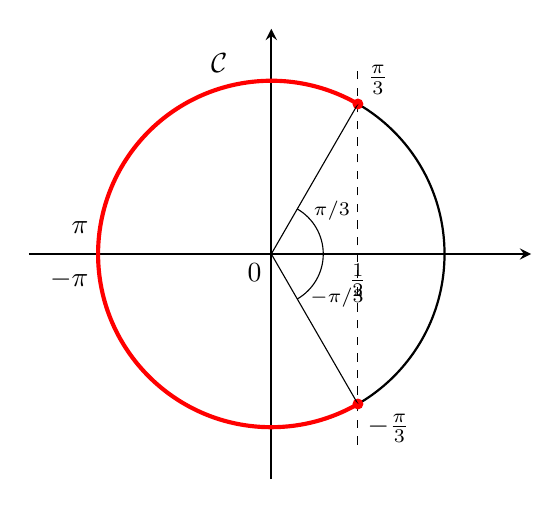
\begin{tikzpicture}[scale=2.2, >=stealth]
    % Axes
    \draw[->, thick] (-1.4,0) -- (1.5,0);
    \draw[->, thick] (0,-1.3) -- (0,1.3);
    
    % Cercle trigonométrique
    \draw[thick] (0,0) circle (1);
    \node at (-0.3, 1.1) {$\mathcal{C}$};
    
    % Origine
    \node[below left] at (0,0) {$0$};
    
    % Point 1/2 sur l'axe des abscisses
    \draw[dashed] (0.5,-1.1) -- (0.5,1.1);
    \node[below] at (0.5,0) {$\frac{1}{2}$};
    
    % Points pi/3 et -pi/3
    \filldraw[red] (0.5, 0.866) circle (0.8pt);
    \filldraw[red] (0.5, -0.866) circle (0.8pt);
    
    \draw (0,0) -- (0.5, 0.866) node[above right] {$\frac{\pi}{3}$};
    \draw (0,0) -- (0.5, -0.866) node[below right] {$-\frac{\pi}{3}$};
    
    % Angles
    \draw (0.3,0) arc (0:60:0.3);
    \node at (0.35, 0.25) {\scriptsize $\pi/3$};
    
    \draw (0.3,0) arc (0:-60:0.3);
    \node at (0.38, -0.25) {\scriptsize $-\pi/3$};
    
    % Points -pi et pi
    \node[left] at (-1, 0.15) {$\pi$};
    \node[left] at (-1, -0.15) {$-\pi$};
    
    % Arc des solutions (surbrillance)
    \draw[line width=1.5pt, red] (0.5, 0.866) arc (60:180:1);
    \draw[line width=1.5pt, red] (-1,0) arc (180:300:1);
\end{tikzpicture}
\end{center}

\[
S = \left] -\pi\,;\, -\frac{\pi}{3} \right] \cup \left[ \frac{\pi}{3}\,;\, \pi \right]
\]

\begin{center}
    \underline{\textbf{\Large Autre méthode}}
\end{center}

\vspace{0.3cm}

\noindent Étudions le signe de $\cos x - \dfrac{1}{2}$ dans $]-\pi, \pi]$ :

\vspace{0.3cm}

Posons $\cos x - \dfrac{1}{2} = 0 \iff \cos x = \dfrac{1}{2}$

\hspace{3.4cm} $\iff x = \dfrac{\pi}{3} \text{ ou } x = -\dfrac{\pi}{3}$

\vspace{0.5cm}

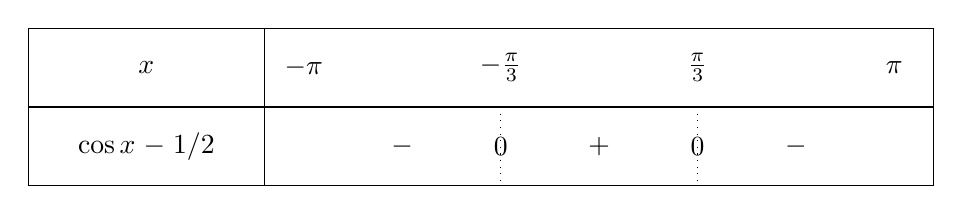
\begin{tikzpicture}
   \tkzTabInit[lgt=3, espcl=2.5]{$x$ / 1 , {$\cos x - 1/2$} / 1}{$-\pi$, $-\frac{\pi}{3}$, $\frac{\pi}{3}$, $\pi$}
   \tkzTabLine{, -, z, +, z, -, }
\end{tikzpicture}

\[
S = \left] -\pi \,;\, -\frac{\pi}{3} \right] \cup \left[ \frac{\pi}{3} \,;\, \pi \right]
\]

\paragraph{\Large\textbf{Application :}} Résoudre dans $\mathbb{R}$

\vspace{0.3cm}

\begin{multicols}{2}
\begin{enumerate}
    \item $\cos x = \frac{-\sqrt{3}}{2}$
    \item $\cos 2x = \cos(\pi + 4x)$
    \item $\cos x = \frac{1+\sqrt{2}}{2}$
    \item $\sin x = \frac{\sqrt{3}}{2}$
    \item $\sin(x - \pi) = \sin 3x$
    \item $\sin x = \frac{1-2\sqrt{3}}{2}$
    \item $\tan x = \frac{\sqrt{3}}{2}$
    \item $\tan(-2x) = \tan(\pi - 3x)$
    \item $\tan x = \frac{\sqrt{3}}{3}$
    \item $\cos x + \sin x = \sqrt{2}$
    \item $\sin x \ge \frac{1}{2}$ dans $]-\pi, \pi[$
    \item $\cos x \le -\frac{1}{2}$ dans $[-2\pi, 2\pi]$
    \item $\tan x \ge \sqrt{3}$ dans $]-\pi, \pi[$
    \item $\tan x \le -\frac{1}{2}$ dans $[-2\pi, 2\pi]$
\end{enumerate}
\end{multicols}
\end{document}